
\begin{alphasection}

\section{Introduksjon - Praktisk rundt laben}
I heisprosjektet skal dere bruke det dere har lært i de tidligere fem øvingene til å samarbeide om et større prosjekt, altså til utviklingen av programvare for logikkstyring av et fysisk system, i dette tilfellet en heismodell.

Som dere vet, er programmeringsspråket \verb|C| et kraftig verktøy som regelmessig benyttes i et bredt spekter av industri-sammenhenger, særlig i sanntidsapplikasjoner og maskinnær programvare. Denne laben går ut på å benytte \verb|C| til å implementere et styresystem for en fysisk heis-modell på Sanntidssalen (se introduksjon \ref{sec:2-innføringheis}), som styres gjennom en Arduino. I tillegg til selve implementasjonen, skal systemet beskrives og dokumenteres med UML før dere starter med selve implementasjonen.

For å strukturere arbeidet, og sikre verifikasjon av akseptkriterier, skal den pragmatiske V-modellen benyttes (se appendiks \ref{app:vmodell}), og den tilhørende rapporten skal speile dette. Flittig bruk av \verb|git| vil gjøre utførelsen av prosjektet enklere, og selv om dette ikke er obligatorisk, så er det anbefalt å bruke \verb|git| sammen med en kodevertsplattform slik som GitHub. Ettersom dere skal følge den pragmatiske V-modellen i dette prosjektet, er det derfor lurt at \verb|git|-historikken speiler dette.

\subsection*{Godkjenning}

Heis-laben vil ikke telle på sluttkarakteren i år, men må godkjennes for at dere skal kunne gå opp til eksamen. Prosjektet er konseptuelt delt i 3 deler (oppgaver), som i utgangspunktet må godkjennes:
\begin{itemize}
    \item UML-del med klasse-, sekvens og tilstands-diagrammer. Dere skal her strukturere heis-prosjektet med ulike diagrammer for å beskrive implementasjonen før den blir skrevet.
    \item Implementasjons-del med en FAT (\textbf{F}actory \textbf{A}cceptance \textbf{T}est) (se appendiks \ref{subsec:FAT}). Dette er for å se at implementasjonen faktisk oppfører seg som en heis.
    \item Refleksjon rundt egen implementasjon og hvordan det har vært å bruke UML og V-modellen, og hvordan bruken av disse har påvirket implementasjonen. Dersom dere har brukt generative KI-verktøy slik som ChatGPT i arbeidet med heisprosjektet, så skal dette også dokumenteres. Se appendiks \ref{app:refleksjon} for kommentar på de viktigste punktene.
\end{itemize}

God bruk av \verb|git| og dokumentering av kode med \verb|doxygen| er ikke obligatorisk, men begge deler vil gjøre arbeidet med heisprosjektet enklere for dere, samtidig som dette er nyttige verktøy å mestre til senere arbeid. I tillegg vil begge disse delene telle positivt for prosjektet, og kunne trekke dere opp dersom det finnes andre mangler ved prosjektet deres.

UML- og refleksjonsdelen inngår i en rapport som dere skal skrive. Denne skal være på maks ti sider, inkludert alt av figurer, og kan skrives på norsk, engelsk eller tysk. Denne skal inneholde alle de tidligere nevnte kravene, samt alt annet som trengs for å beskrive prosjektet deres. Denne rapporten leveres på BlackBoard sammen med all kildekoden deres, altså alt som trengs for å kunne gjenskape resultatene fra FATen.

\subsection*{Viktige datoer}
Som man kan se fra tabell \ref{tab:viktige-dato}, så blir FAT-en utført i uke 11. Dette vil foregå på Sanntidssalen hvor tidspunkt avhenger av når dere har saltid. Det eneste dere trenger å gjøre er å vente på arbeidsplassene deres, så vil studass eller vitass komme til arbeidsplassene deres og utføre FAT-en med styresystemet deres. Rapporten og koden deres leveres inn på Blackboard som en zip-fil uken etter.

\begin{table}[ht]
\centering
 \begin{tabular}{|p{4cm} p{5.5cm}|} 
 \hline
 Viktige dato & Beskrivelse \\ [0.5ex] 
 \hline\hline
  Labtid, uke 11 & FAT \\
 \hline
  Fredag 22. mars & Rapport + kode som zip-fil \\
 \hline
\end{tabular}
\caption{Viktige datoer å merke}
\label{tab:viktige-dato} 
\end{table}

\section{Introduksjon - Praktisk rundt de utleverte filene}

I denne laben får dere utlevert noen \verb|.c| og \verb|.h|-filer under \verb|skeleton_project|-mappen. Tabellen under lister opp alle filene som blir utlevert til bruk i heisprosjektet, samt litt informasjon om dere skal endre på filene eller om dere skal la dem bli i løpet av øvingen. I kontekst av tabellen under, så betyr \textit{helst ikke} at dere kan endre på filene, men at dette ikke burde gjøres siden det kan føre til andre komplikasjoner videre på veien. For eksempel: om det trengs mer kompliserte funksjoner enn de som allerede er definert i \verb|elevio|, så anbefales det å opprette filer som bruker de allerede definerte funksjonene i \verb|elevio| istedenfor å endre direkte på \verb|elevio|-funksjonene.

\begin{center}
 \begin{tabular}{|p{8.5cm} p{5.5cm}|} 
 \hline
 Filer & Skal filen(e) endres?  \\ [0.5ex] 
 \hline\hline
  \verb|skeleton_project/Makefile| & \quad \quad \quad \quad Ja \\
 \hline
   \verb|skeleton_project/SimElevatorServer| & \quad \quad \quad \quad Nei \\
 \hline
   \verb|skeleton_project/SimElevatorServer.exe| & \quad \quad \quad \quad Nei \\
 \hline
   \verb|skeleton_project/simulator.con| & \quad \quad \quad \quad Nei \\
 \hline
  \verb|skeleton_project/source/main.c| & \quad \quad \quad \quad Ja  \\ 
 \hline
  \verb|skeleton_project/source/driver/elevio.c| &  \quad \quad \quad \quad Helst ikke \\ 
 \hline
 \verb|skeleton_project/source/driver/elevio.h| &  \quad \quad \quad \quad Helst ikke \\ 
 \hline
  \verb|skeleton_project/source/driver/elevio.con| &  \quad \quad \quad \quad Nei \\ 
 \hline
  \verb|skeleton_project/source/driver/con_load.h| &  \quad \quad \quad \quad Nei \\ 
 \hline
 \verb|skeleton_project/source/driver/elev_test.c| &  \quad \quad \quad \quad Nei \\
  \hline
 \verb|Main/*| & \quad \quad \quad \quad Nei  \\ 
 \hline
 \verb|.github/*| & \quad \quad \quad \quad Nei \\
 \hline 
\end{tabular}
\end{center}

\clearpage

\section{Introduksjon - Heisen på sanntidslaben}\label{sec:2-innføringheis}

Vi skal bruke en fysisk modell av en heis i løpet av prosjektet som skal styres med et styringssystem ved hjelp av en Arduino. heis-modellen består av tre hoveddeler; selve heismodellen, et betjeningspanel, og en motorstyringsboks. Det finnes en heis-modell på nesten hver av sanntidssalens arbeidsplasser. Hensikten med denne laben er at dere skal programmere oppførselen til heisen med \verb|C| uten å måtte ta hensyn til minnebegrensninger (Minnehåndtering i mikrokontrollere blir introdusert i mikrokontroller-laben).



\subsection{Heis-modell}
Heis-modellen er illustrert i figur \ref{fig:heis-modell-sal} og består av en heisstol som kan beveges opp og ned langs en stolpe. Dette tilsvarer henholdsvis heisrommet- og sjakten i en virkelig heis.

\begin{figure}[ht]
    \centering
    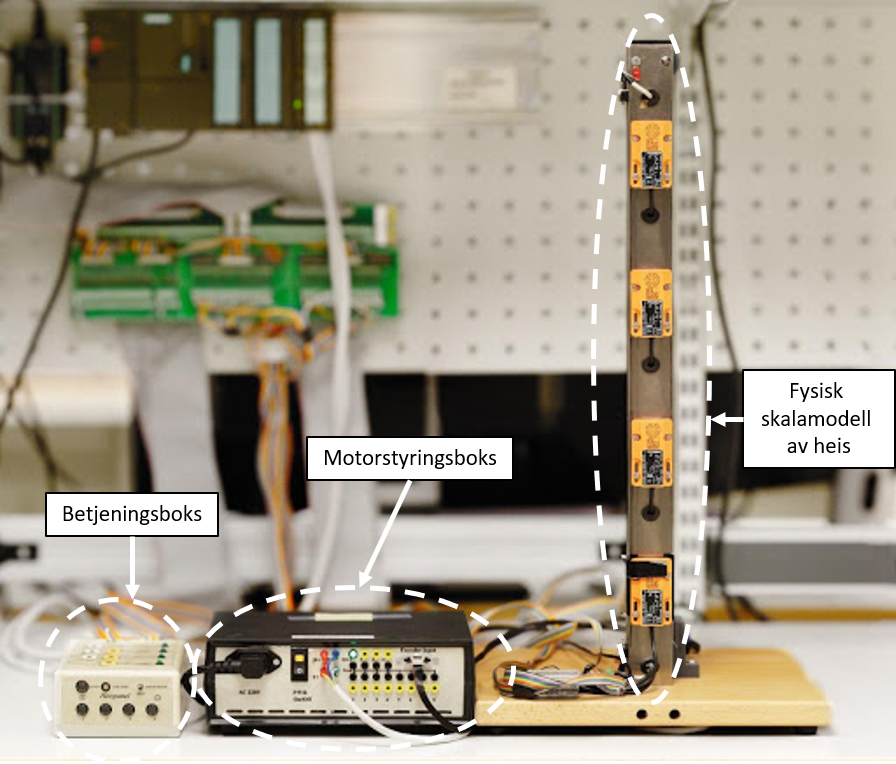
\includegraphics[scale=.85]{figures/HEIS.png}
    \caption{Heis-modellen på sanntidslaben.}
    \label{fig:heis-modell-sal}
\end{figure}

Langs heisbanen er det montert fire hall-effektsensorer som fungerer som heisens etasjer. Over øverste etasje, og under nederste etasje er det også montert endestoppbrytere, som vil kutte motorpådraget dersom heisen kjører utenfor sitt lovlige område. Dette er for å beskytte heisens motor mot skade. Om heisen skulle treffe en av endestoppene, må heisstolen manuelt skyves bort fra bryterne før en kan be motoren om et nytt pådrag.

\subsection{Betjeningsboks}
Betjenings-boksen er delt i to; \textit{etasjepanel} og \textit{heispanel}. Disse kan man finne i figur \ref{fig:heis-modell-sal} og \ref{fig:paneler}. Øverst på betjeningsboksen finnes en bryter som velger om datamaskinen eller PLSen skal styre heismodellen. Denne skal stå i \verb|PC| gjennom hele laben.

\begin{figure}[ht]
    \centering
    



\tikzset{every picture/.style={line width=0.75pt}} %set default line width to 0.75pt        

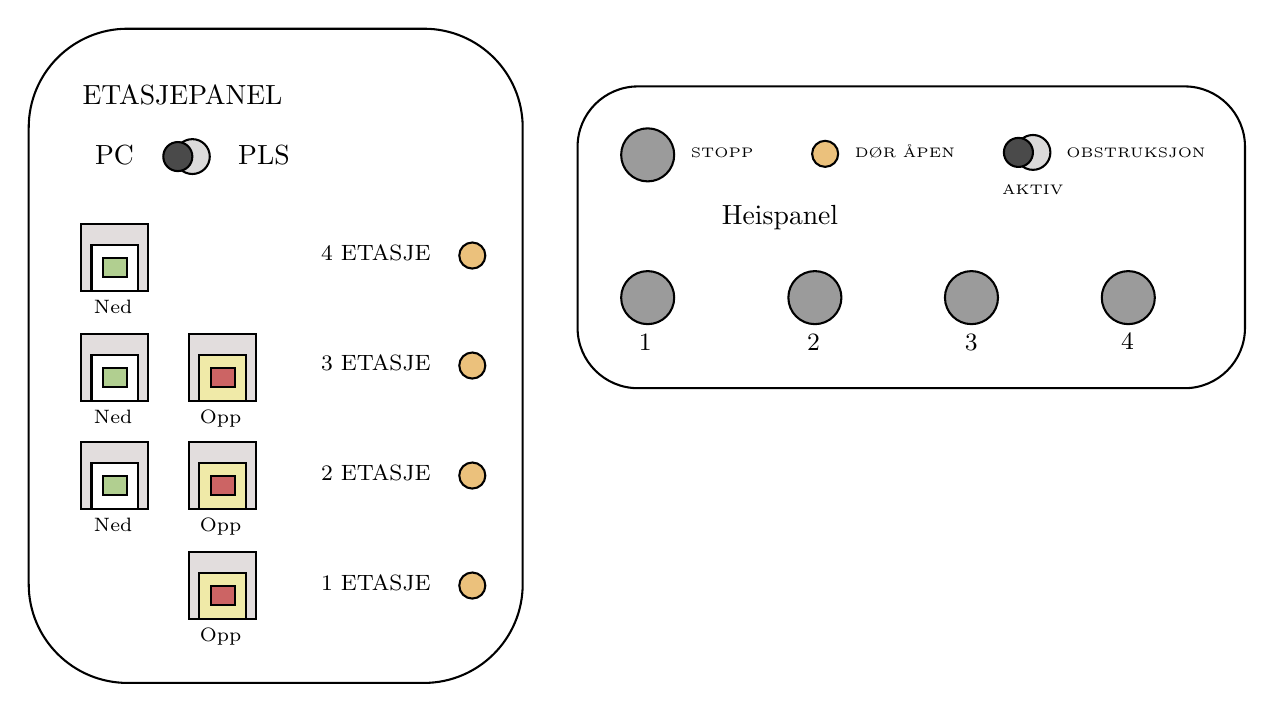
\begin{tikzpicture}[x=0.75pt,y=0.75pt,yscale=-1,xscale=1]
%uncomment if require: \path (0,386); %set diagram left start at 0, and has height of 386

%Rounded Rect [id:dp9950110832791259] 
\draw   (47.56,88.6) .. controls (47.56,62.31) and (68.87,41) .. (95.16,41) -- (237.96,41) .. controls (264.25,41) and (285.56,62.31) .. (285.56,88.6) -- (285.56,308.6) .. controls (285.56,334.89) and (264.25,356.2) .. (237.96,356.2) -- (95.16,356.2) .. controls (68.87,356.2) and (47.56,334.89) .. (47.56,308.6) -- cycle ;
%Shape: Circle [id:dp32702530949930675] 
\draw  [fill={rgb, 255:red, 219; green, 218; blue, 218 }  ,fill opacity=1 ] (118,102.6) .. controls (118,97.96) and (121.76,94.2) .. (126.4,94.2) .. controls (131.04,94.2) and (134.8,97.96) .. (134.8,102.6) .. controls (134.8,107.24) and (131.04,111) .. (126.4,111) .. controls (121.76,111) and (118,107.24) .. (118,102.6) -- cycle ;
%Shape: Circle [id:dp5550022005610891] 
\draw  [fill={rgb, 255:red, 74; green, 74; blue, 74 }  ,fill opacity=1 ] (112.4,102.6) .. controls (112.4,98.73) and (115.53,95.6) .. (119.4,95.6) .. controls (123.27,95.6) and (126.4,98.73) .. (126.4,102.6) .. controls (126.4,106.47) and (123.27,109.6) .. (119.4,109.6) .. controls (115.53,109.6) and (112.4,106.47) .. (112.4,102.6) -- cycle ;
%Rounded Rect [id:dp07742975412184872] 
\draw   (312,97.88) .. controls (312,81.82) and (325.02,68.8) .. (341.08,68.8) -- (604.48,68.8) .. controls (620.54,68.8) and (633.56,81.82) .. (633.56,97.88) -- (633.56,185.12) .. controls (633.56,201.18) and (620.54,214.2) .. (604.48,214.2) -- (341.08,214.2) .. controls (325.02,214.2) and (312,201.18) .. (312,185.12) -- cycle ;
%Shape: Circle [id:dp5584647222054995] 
\draw  [fill={rgb, 255:red, 155; green, 155; blue, 155 }  ,fill opacity=1 ] (333,101.78) .. controls (333,94.72) and (338.72,89) .. (345.78,89) .. controls (352.84,89) and (358.56,94.72) .. (358.56,101.78) .. controls (358.56,108.84) and (352.84,114.56) .. (345.78,114.56) .. controls (338.72,114.56) and (333,108.84) .. (333,101.78) -- cycle ;
%Shape: Circle [id:dp36378536676727435] 
\draw  [fill={rgb, 255:red, 235; green, 193; blue, 124 }  ,fill opacity=1 ] (425,101.28) .. controls (425,97.81) and (427.81,95) .. (431.28,95) .. controls (434.75,95) and (437.56,97.81) .. (437.56,101.28) .. controls (437.56,104.75) and (434.75,107.56) .. (431.28,107.56) .. controls (427.81,107.56) and (425,104.75) .. (425,101.28) -- cycle ;
%Shape: Circle [id:dp2626490795793748] 
\draw  [fill={rgb, 255:red, 219; green, 218; blue, 218 }  ,fill opacity=1 ] (523,100.6) .. controls (523,95.96) and (526.76,92.2) .. (531.4,92.2) .. controls (536.04,92.2) and (539.8,95.96) .. (539.8,100.6) .. controls (539.8,105.24) and (536.04,109) .. (531.4,109) .. controls (526.76,109) and (523,105.24) .. (523,100.6) -- cycle ;
%Shape: Circle [id:dp7325663462799819] 
\draw  [fill={rgb, 255:red, 74; green, 74; blue, 74 }  ,fill opacity=1 ] (517.4,100.6) .. controls (517.4,96.73) and (520.53,93.6) .. (524.4,93.6) .. controls (528.27,93.6) and (531.4,96.73) .. (531.4,100.6) .. controls (531.4,104.47) and (528.27,107.6) .. (524.4,107.6) .. controls (520.53,107.6) and (517.4,104.47) .. (517.4,100.6) -- cycle ;

%Shape: Circle [id:dp3804510595811603] 
\draw  [fill={rgb, 255:red, 155; green, 155; blue, 155 }  ,fill opacity=1 ] (333,170.56) .. controls (333,163.5) and (338.72,157.78) .. (345.78,157.78) .. controls (352.84,157.78) and (358.56,163.5) .. (358.56,170.56) .. controls (358.56,177.62) and (352.84,183.34) .. (345.78,183.34) .. controls (338.72,183.34) and (333,177.62) .. (333,170.56) -- cycle ;
%Shape: Circle [id:dp9317202699472626] 
\draw  [fill={rgb, 255:red, 155; green, 155; blue, 155 }  ,fill opacity=1 ] (413.56,170.56) .. controls (413.56,163.5) and (419.28,157.78) .. (426.34,157.78) .. controls (433.4,157.78) and (439.12,163.5) .. (439.12,170.56) .. controls (439.12,177.62) and (433.4,183.34) .. (426.34,183.34) .. controls (419.28,183.34) and (413.56,177.62) .. (413.56,170.56) -- cycle ;
%Shape: Circle [id:dp8967657062909633] 
\draw  [fill={rgb, 255:red, 155; green, 155; blue, 155 }  ,fill opacity=1 ] (489,170.56) .. controls (489,163.5) and (494.72,157.78) .. (501.78,157.78) .. controls (508.84,157.78) and (514.56,163.5) .. (514.56,170.56) .. controls (514.56,177.62) and (508.84,183.34) .. (501.78,183.34) .. controls (494.72,183.34) and (489,177.62) .. (489,170.56) -- cycle ;
%Shape: Circle [id:dp46875668862956843] 
\draw  [fill={rgb, 255:red, 155; green, 155; blue, 155 }  ,fill opacity=1 ] (564.56,170.56) .. controls (564.56,163.5) and (570.28,157.78) .. (577.34,157.78) .. controls (584.4,157.78) and (590.12,163.5) .. (590.12,170.56) .. controls (590.12,177.62) and (584.4,183.34) .. (577.34,183.34) .. controls (570.28,183.34) and (564.56,177.62) .. (564.56,170.56) -- cycle ;
%Shape: Circle [id:dp6506882141668844] 
\draw  [fill={rgb, 255:red, 235; green, 193; blue, 124 }  ,fill opacity=1 ] (255,150.28) .. controls (255,146.81) and (257.81,144) .. (261.28,144) .. controls (264.75,144) and (267.56,146.81) .. (267.56,150.28) .. controls (267.56,153.75) and (264.75,156.56) .. (261.28,156.56) .. controls (257.81,156.56) and (255,153.75) .. (255,150.28) -- cycle ;
%Shape: Circle [id:dp7349408120329506] 
\draw  [fill={rgb, 255:red, 235; green, 193; blue, 124 }  ,fill opacity=1 ] (255,203.28) .. controls (255,199.81) and (257.81,197) .. (261.28,197) .. controls (264.75,197) and (267.56,199.81) .. (267.56,203.28) .. controls (267.56,206.75) and (264.75,209.56) .. (261.28,209.56) .. controls (257.81,209.56) and (255,206.75) .. (255,203.28) -- cycle ;
%Shape: Circle [id:dp08591264771647289] 
\draw  [fill={rgb, 255:red, 235; green, 193; blue, 124 }  ,fill opacity=1 ] (255,256.28) .. controls (255,252.81) and (257.81,250) .. (261.28,250) .. controls (264.75,250) and (267.56,252.81) .. (267.56,256.28) .. controls (267.56,259.75) and (264.75,262.56) .. (261.28,262.56) .. controls (257.81,262.56) and (255,259.75) .. (255,256.28) -- cycle ;
%Shape: Circle [id:dp13492097445361106] 
\draw  [fill={rgb, 255:red, 235; green, 193; blue, 124 }  ,fill opacity=1 ] (255,309.28) .. controls (255,305.81) and (257.81,303) .. (261.28,303) .. controls (264.75,303) and (267.56,305.81) .. (267.56,309.28) .. controls (267.56,312.75) and (264.75,315.56) .. (261.28,315.56) .. controls (257.81,315.56) and (255,312.75) .. (255,309.28) -- cycle ;
%Shape: Square [id:dp9156786654213831] 
\draw  [fill={rgb, 255:red, 226; green, 221; blue, 221 }  ,fill opacity=1 ] (72.8,135) -- (105,135) -- (105,167.2) -- (72.8,167.2) -- cycle ;
%Shape: Rectangle [id:dp9366523430197387] 
\draw  [color={rgb, 255:red, 0; green, 0; blue, 0 }  ,draw opacity=1 ][fill={rgb, 255:red, 255; green, 255; blue, 255 }  ,fill opacity=1 ] (77.8,145.2) -- (100.24,145.2) -- (100.24,167.2) -- (77.8,167.2) -- cycle ;
%Shape: Rectangle [id:dp17647947769063999] 
\draw  [fill={rgb, 255:red, 177; green, 207; blue, 144 }  ,fill opacity=1 ] (83.24,151.6) -- (94.8,151.6) -- (94.8,160.8) -- (83.24,160.8) -- cycle ;
%Shape: Square [id:dp3110641273660344] 
\draw  [fill={rgb, 255:red, 226; green, 221; blue, 221 }  ,fill opacity=1 ] (124.8,188) -- (157,188) -- (157,220.2) -- (124.8,220.2) -- cycle ;
%Shape: Rectangle [id:dp3411082188269683] 
\draw  [fill={rgb, 255:red, 240; green, 234; blue, 168 }  ,fill opacity=1 ] (129.8,198.2) -- (152.24,198.2) -- (152.24,220.2) -- (129.8,220.2) -- cycle ;
%Shape: Rectangle [id:dp024921669891114773] 
\draw  [fill={rgb, 255:red, 204; green, 100; blue, 100 }  ,fill opacity=1 ] (135.24,204.6) -- (146.8,204.6) -- (146.8,213.8) -- (135.24,213.8) -- cycle ;
%Shape: Square [id:dp802085856449118] 
\draw  [fill={rgb, 255:red, 226; green, 221; blue, 221 }  ,fill opacity=1 ] (124.8,240) -- (157,240) -- (157,272.2) -- (124.8,272.2) -- cycle ;
%Shape: Rectangle [id:dp5915145699519246] 
\draw  [fill={rgb, 255:red, 240; green, 234; blue, 168 }  ,fill opacity=1 ] (129.8,250.2) -- (152.24,250.2) -- (152.24,272.2) -- (129.8,272.2) -- cycle ;
%Shape: Rectangle [id:dp03960973210916041] 
\draw  [fill={rgb, 255:red, 204; green, 100; blue, 100 }  ,fill opacity=1 ] (135.24,256.6) -- (146.8,256.6) -- (146.8,265.8) -- (135.24,265.8) -- cycle ;
%Shape: Square [id:dp831298532737776] 
\draw  [fill={rgb, 255:red, 226; green, 221; blue, 221 }  ,fill opacity=1 ] (124.8,293) -- (157,293) -- (157,325.2) -- (124.8,325.2) -- cycle ;
%Shape: Rectangle [id:dp15467787894146512] 
\draw  [fill={rgb, 255:red, 240; green, 234; blue, 168 }  ,fill opacity=1 ] (129.8,303.2) -- (152.24,303.2) -- (152.24,325.2) -- (129.8,325.2) -- cycle ;
%Shape: Rectangle [id:dp34679432751904793] 
\draw  [fill={rgb, 255:red, 204; green, 100; blue, 100 }  ,fill opacity=1 ] (135.24,309.6) -- (146.8,309.6) -- (146.8,318.8) -- (135.24,318.8) -- cycle ;
%Shape: Square [id:dp4723272264815428] 
\draw  [fill={rgb, 255:red, 226; green, 221; blue, 221 }  ,fill opacity=1 ] (72.8,240) -- (105,240) -- (105,272.2) -- (72.8,272.2) -- cycle ;
%Shape: Rectangle [id:dp07462637657852489] 
\draw  [color={rgb, 255:red, 0; green, 0; blue, 0 }  ,draw opacity=1 ][fill={rgb, 255:red, 255; green, 255; blue, 255 }  ,fill opacity=1 ] (77.8,250.2) -- (100.24,250.2) -- (100.24,272.2) -- (77.8,272.2) -- cycle ;
%Shape: Rectangle [id:dp5263621720064795] 
\draw  [fill={rgb, 255:red, 177; green, 207; blue, 144 }  ,fill opacity=1 ] (83.24,256.6) -- (94.8,256.6) -- (94.8,265.8) -- (83.24,265.8) -- cycle ;
%Shape: Square [id:dp4171956285217089] 
\draw  [fill={rgb, 255:red, 226; green, 221; blue, 221 }  ,fill opacity=1 ] (72.8,188) -- (105,188) -- (105,220.2) -- (72.8,220.2) -- cycle ;
%Shape: Rectangle [id:dp8897782495872741] 
\draw  [color={rgb, 255:red, 0; green, 0; blue, 0 }  ,draw opacity=1 ][fill={rgb, 255:red, 255; green, 255; blue, 255 }  ,fill opacity=1 ] (77.8,198.2) -- (100.24,198.2) -- (100.24,220.2) -- (77.8,220.2) -- cycle ;
%Shape: Rectangle [id:dp3645531927882917] 
\draw  [fill={rgb, 255:red, 177; green, 207; blue, 144 }  ,fill opacity=1 ] (83.24,204.6) -- (94.8,204.6) -- (94.8,213.8) -- (83.24,213.8) -- cycle ;

% Text Node
\draw (72,67) node [anchor=north west][inner sep=0.75pt]   [align=left] {ETASJEPANEL};
% Text Node
\draw (78,96) node [anchor=north west][inner sep=0.75pt]   [align=left] {PC};
% Text Node
\draw (147,96) node [anchor=north west][inner sep=0.75pt]   [align=left] {PLS};
% Text Node
\draw (380.05,124.81) node [anchor=north west][inner sep=0.75pt]   [align=left] {Heispanel};
% Text Node
\draw (444.05,95.7) node [anchor=north west][inner sep=0.75pt]  [font=\tiny] [align=left] {DØR ÅPEN};
% Text Node
\draw (546.05,97) node [anchor=north west][inner sep=0.75pt]  [font=\tiny] [align=left] {OBSTRUKSJON};
% Text Node
\draw (365.05,97) node [anchor=north west][inner sep=0.75pt]  [font=\tiny] [align=left] {STOPP};
% Text Node
\draw (515.05,114.81) node [anchor=north west][inner sep=0.75pt]  [font=\tiny] [align=left] {AKTIV};
% Text Node
\draw (340.05,186.81) node [anchor=north west][inner sep=0.75pt]  [font=\small] [align=left] {1};
% Text Node
\draw (421.05,186.81) node [anchor=north west][inner sep=0.75pt]  [font=\small] [align=left] {2};
% Text Node
\draw (497.05,186.81) node [anchor=north west][inner sep=0.75pt]  [font=\small] [align=left] {3};
% Text Node
\draw (572.34,186.34) node [anchor=north west][inner sep=0.75pt]  [font=\small] [align=left] {4};
% Text Node
\draw (187,144) node [anchor=north west][inner sep=0.75pt]  [font=\footnotesize] [align=left] {4 ETASJE};
% Text Node
\draw (187,197) node [anchor=north west][inner sep=0.75pt]  [font=\footnotesize] [align=left] {3 ETASJE};
% Text Node
\draw (187,250) node [anchor=north west][inner sep=0.75pt]  [font=\footnotesize] [align=left] {2 ETASJE};
% Text Node
\draw (187,303) node [anchor=north west][inner sep=0.75pt]  [font=\footnotesize] [align=left] {1 ETASJE};
% Text Node
\draw (77.5,170.2) node [anchor=north west][inner sep=0.75pt]  [font=\scriptsize] [align=left] {Ned};
% Text Node
\draw (77.5,223.2) node [anchor=north west][inner sep=0.75pt]  [font=\scriptsize] [align=left] {Ned};
% Text Node
\draw (77.5,275.2) node [anchor=north west][inner sep=0.75pt]  [font=\scriptsize] [align=left] {Ned};
% Text Node
\draw (128.5,223.2) node [anchor=north west][inner sep=0.75pt]  [font=\scriptsize] [align=left] {Opp};
% Text Node
\draw (128.5,275.2) node [anchor=north west][inner sep=0.75pt]  [font=\scriptsize] [align=left] {Opp};
% Text Node
\draw (128.5,328.2) node [anchor=north west][inner sep=0.75pt]  [font=\scriptsize] [align=left] {Opp};


\end{tikzpicture}
    \caption{Etasje- og Heispanel i sanntidslaben}
    \label{fig:paneler}
\end{figure}

Etasjepanelet finnes på oversiden av betjeningsboksen. På dette panelet finner dere bestillingsknapper for opp- og nedretning fra hver etasje. Hver av knappene er utstyrt med lys som skal indikere om en bestilling er mottatt eller ei. Etasjepanelet har også et lys for hver etasje for å indikere hvilken etasje heisen befinner seg i.

Heispanelet finnes på kortsiden av betjeningsboksen og representerer de knappene man forventer å finne inne i heisrommet til en vanlig heis. Her har man bestillingsknapper for hver etasje, samt en stoppknapp for nødstans. Alle knappene er utstyrt med lys som kan settes via styreprogrammet. I tillegg til knappene er panelet utstyrt med etasjeindikatorlys som kan settes via styreprogrammet og et lys, markert \verb|DØR ÅPEN|, som indikerer om heisdøren er åpen. Heispanelet har også en obstruksjonsbryter, som kan brukes for å simulere at en person blokkerer døren når den er åpen.

\subsection{Motorstyringsboks}

Styringsboksen er ansvarlig for å forsyne effekt til heis-modellen, og for å forsterke pådraget som settes av datamaskinen (se figur \ref{fig:heis-modell-sal}). Motoren kan forsynes med mellom 0- og 5 V, som henholdsvis er minimalt- og maksimalt pådrag. Veien motoren skal gå settes ved et ekstra retningsbit i styringsboksens grensesnitt. Alt dette gjøres via funksjonskall i styringsprogrammet. 

Det er også mulig å hente ut et analogt tacho-signal, samt en digital verdi for motorens encoder, for å lese av hastighet- og posisjon fra styringsboksen. Disse målesignalene trenger dere ikke ta stilling i dette prosjektet, men de nevnes for fullstendighetens skyld.

\subsection{Virkemåte og oppkobling}
Heis-modellen er laget for å konseptuelt oppføre seg som en virkelig heis. Det er et par punkter man bør merke seg for å få den til å fungere som ønsket:

\begin{itemize}
    \item Alle lys må settes eksplisitt. Det er ingen automatikk mellom hall-sensoren i hver etasje og tilhørende etasje-indikator.
    \item Om endestopp-bryterne aktiveres vil pådrag til heisen kuttes. Om det skjer, må heisstolen manuelt skyves vekk fra endestopp.
    
    \item Rød og blå ledning forsyner effekt til motoren. Disse kobles henholdsvis til \textit{M+} og \textit{M-} som dere finner på motorstyringsboksen (se figur \ref{fig:heis-modell-sal}).
    \item Heisen kjøres ved at programmet kompileres med \verb|make|, før styresystemet kjøres med \verb|./elevator|. For at heisen skal ha noe å koble opp i mot, så må man først starte  \verb|elevatorserver|  i et annet terminalvindu først (se figur \ref{fig:terminal-oppstart-heis}).
    \item Dersom man jobber hjemmefra, startes heisen ved at man bruker simulatoren som server istedenfor. Likeså starter man simulatorserveren i et annet terminalvindu først med \verb|./SimElevatorServer|, før man kompilerer og kjører \verb|./elevator| i det opprinnelige terminalvinduet (se appendiks \ref{app:SImulator}).
\end{itemize}

\begin{figure}[ht]
    \centering
    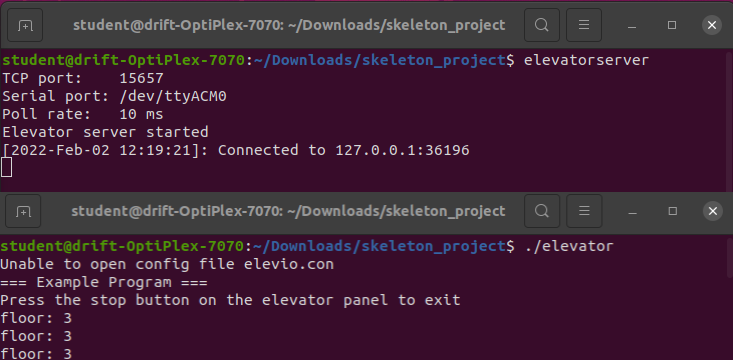
\includegraphics[scale=0.65]{figures/terminal-heis.png}
    \caption{Skjermbilde av terminalene og kommandoene som trengs for å kjøre heisen med utgitt kode.}
    \label{fig:terminal-oppstart-heis}
\end{figure}

% \subsection{Utviklingsmodell og git logg}
% Skal speile V-modellen. Vise at dere har fulgt den.

% \subsection{Oppsett av utviklingsmiljø}
% Henvis til øving 4.
% \subsection{Kommentar til kodekvalitet}

% Et lite appendiks om kodekvalitet har blitt lagt til i appendiks \ref{sec:app-kodekval}. Det er ikke obligatorisk å følge, men kan gjøre videre utvikling lettere med

% \subsection{Bruk av KI-verktøy}
% Kommentar om bruk av KI-verktøy som ChatGPT, Phind ol kommer her. 
% Snakk litt om hallucination leaderboard https://github.com/vectara/hallucination-leaderboard
\end{alphasection}
\clearpage


\setcounter{section}{0}

